\documentclass[conference]{IEEEtran}

\usepackage{graphicx}
\usepackage{amsmath}

\title{Parallel Performance Analysis of $\pi$ Computation using OpenMP}

\author{
\IEEEauthorblockN{Vinaykumar Reddy Junuthula}
\IEEEauthorblockA{CS 7389D: HPC@Scale\\
Texas State University}
}

\begin{document}

\maketitle

\section{Introduction}

Parallel computing plays a critical role in improving the performance of computationally intensive applications. 
This assignment explores the use of OpenMP to parallelize a numerical integration program that computes the value of $\pi$. 
The goal is to evaluate how different OpenMP runtime parameters such as thread placement, thread count, and scheduling policies influence application performance.

\section{System Architecture}

Experiments were performed on a compute node of the Lonestar6 cluster at the Texas Advanced Computing Center (TACC). 
Hardware information was collected using the \texttt{hwloc} and \texttt{lscpu} utilities.

The compute node specifications are summarized below:

\begin{itemize}
\item Processor: AMD EPYC 7763
\item Architecture: x86\_64
\item Total CPUs: 128
\item Sockets: 2
\item Cores per Socket: 64
\item Threads per Core: 1
\item NUMA Nodes: 2
\item L1 Cache: 32 KB
\item L2 Cache: 512 KB
\item L3 Cache: 32 MB
\item CPU Frequency: $\sim$2.45 GHz
\end{itemize}

Because the system contains multiple NUMA nodes, thread placement and scheduling strategies can significantly affect performance.

\section{OpenMP Parallelization}

The sequential program approximates the value of $\pi$ using numerical integration:

\[
\pi = \int_0^1 \frac{4}{1+x^2} dx
\]

The computation is divided into $N$ steps and the function value is evaluated at each step.

To parallelize the program, OpenMP directives were used to distribute loop iterations across threads.

\subsection{OpenMP Constructs}

The following constructs were used:

\begin{itemize}
\item \textbf{\#pragma omp parallel for} – distributes loop iterations among threads.
\item \textbf{reduction(+:sum)} – ensures safe accumulation of partial sums.
\item \textbf{schedule(runtime)} – allows runtime control of scheduling policies.
\end{itemize}

\subsection{Variable Scope}

\begin{itemize}
\item Shared variables: \texttt{num\_steps}, \texttt{step}
\item Private variables: \texttt{i}, \texttt{x}
\item Reduction variable: \texttt{sum}
\end{itemize}

This approach prevents race conditions while enabling efficient parallel execution.

\section{Experimental Results}

All experiments were conducted with:

\[
N = 10,000,000
\]

Execution time was measured using \texttt{omp\_get\_wtime()}.

\subsection{Thread Placement Policies}

The first experiment compared different combinations of OpenMP thread placement parameters:

\begin{itemize}
\item core-close
\item core-spread
\item socket-close
\item socket-spread
\end{itemize}

\begin{figure}[h]
\centering
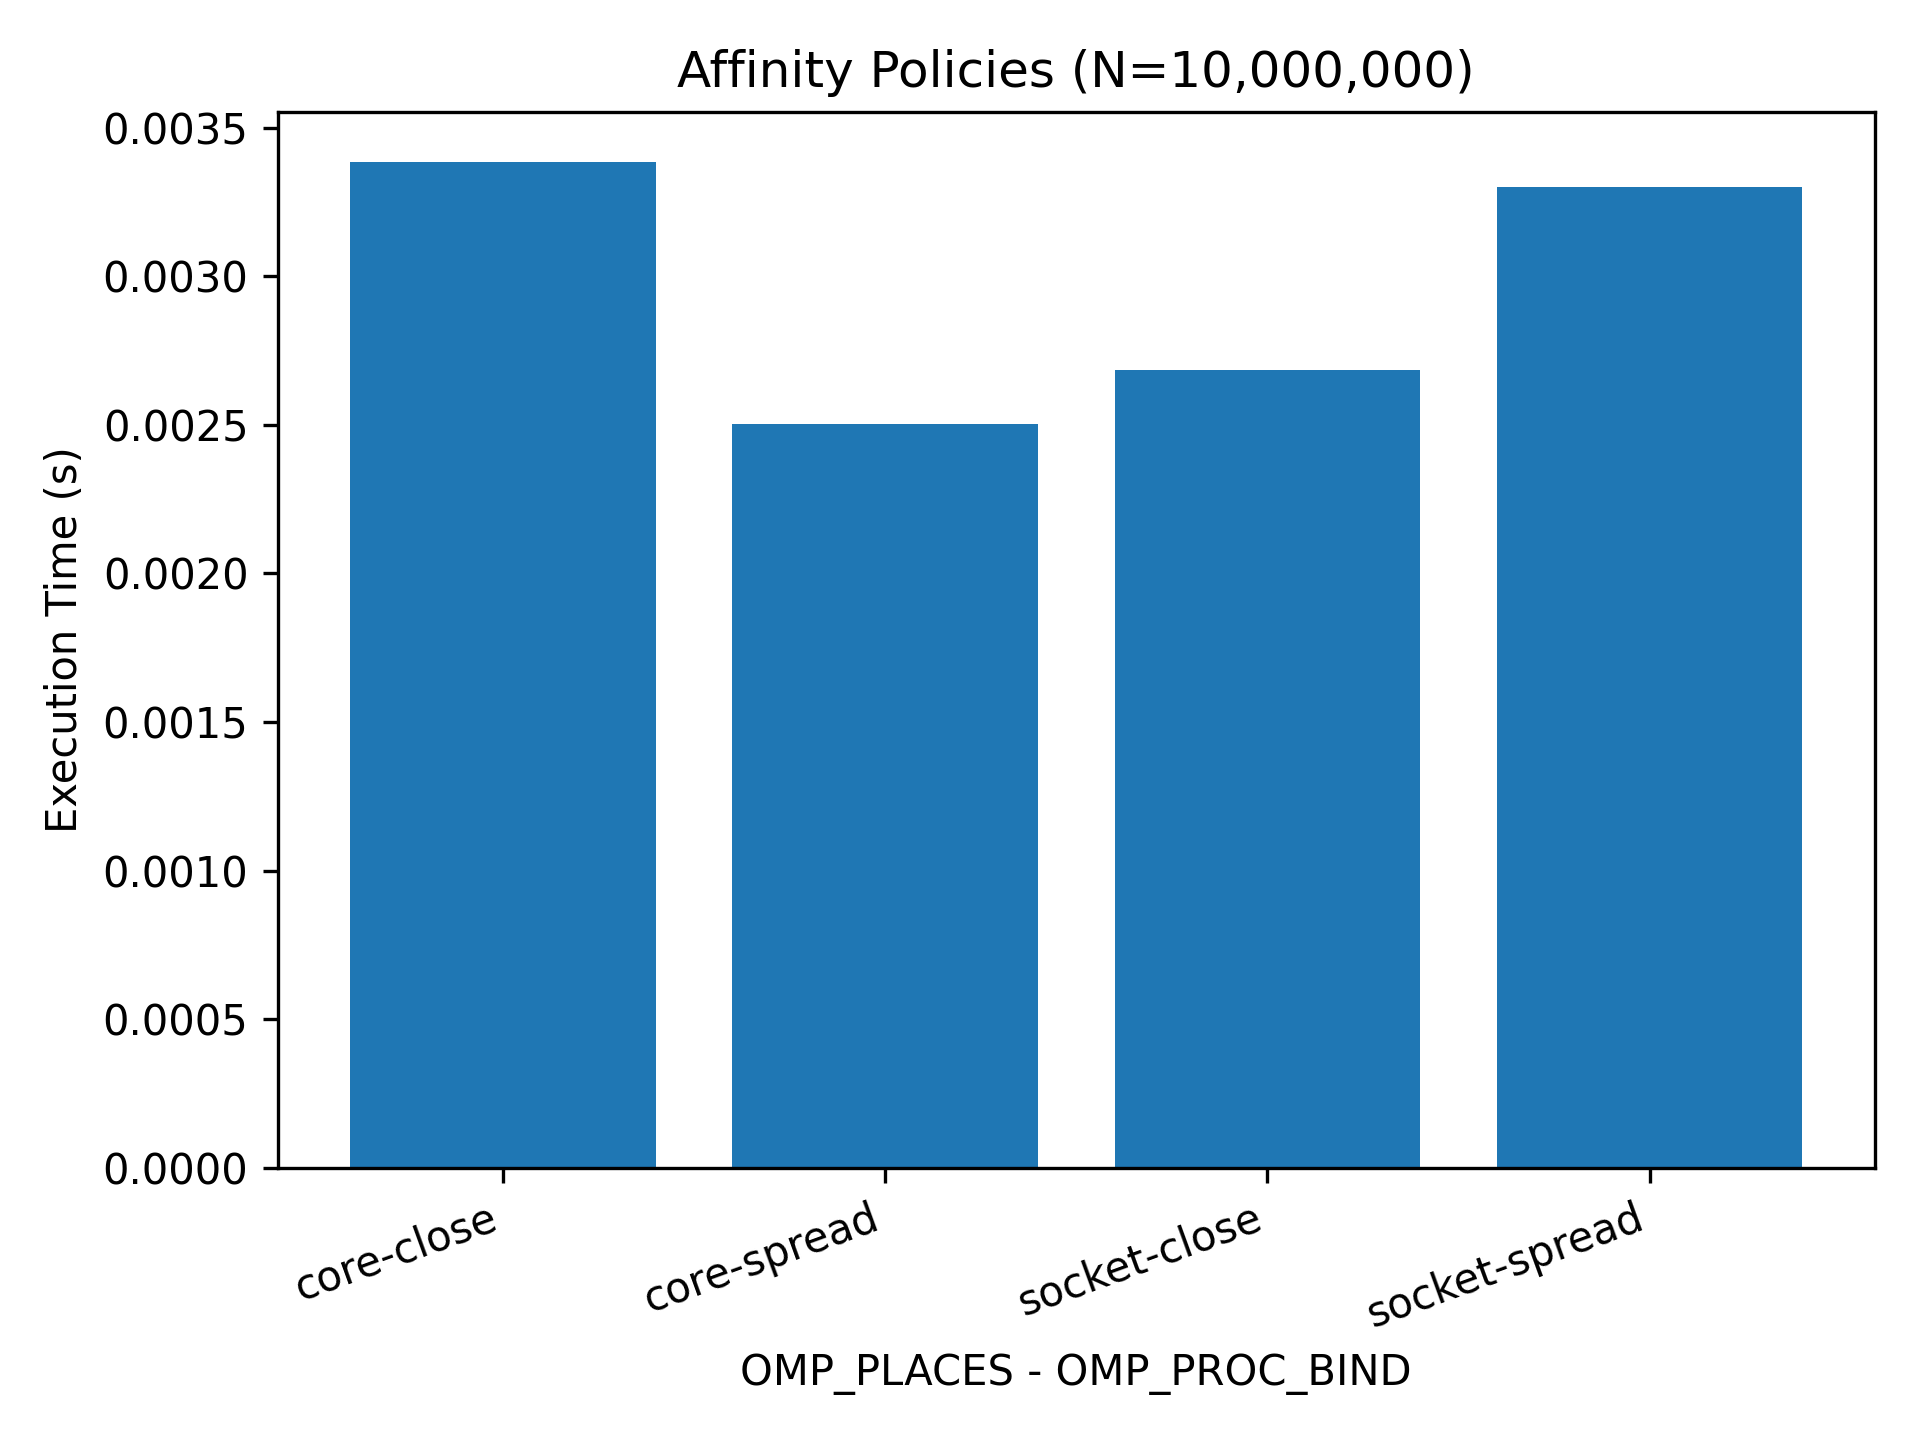
\includegraphics[width=0.45\textwidth]{plot_affinity.png}
\caption{Execution time for different thread placement policies.}
\end{figure}

The results show that \textbf{core-spread} achieved the best performance. 
Spreading threads across cores reduces resource contention and improves overall CPU utilization.

\subsection{Strong Scaling}

The number of threads was varied as:

1, 2, 4, 8, 16, 32, 64, and 128.

\begin{figure}[h]
\centering
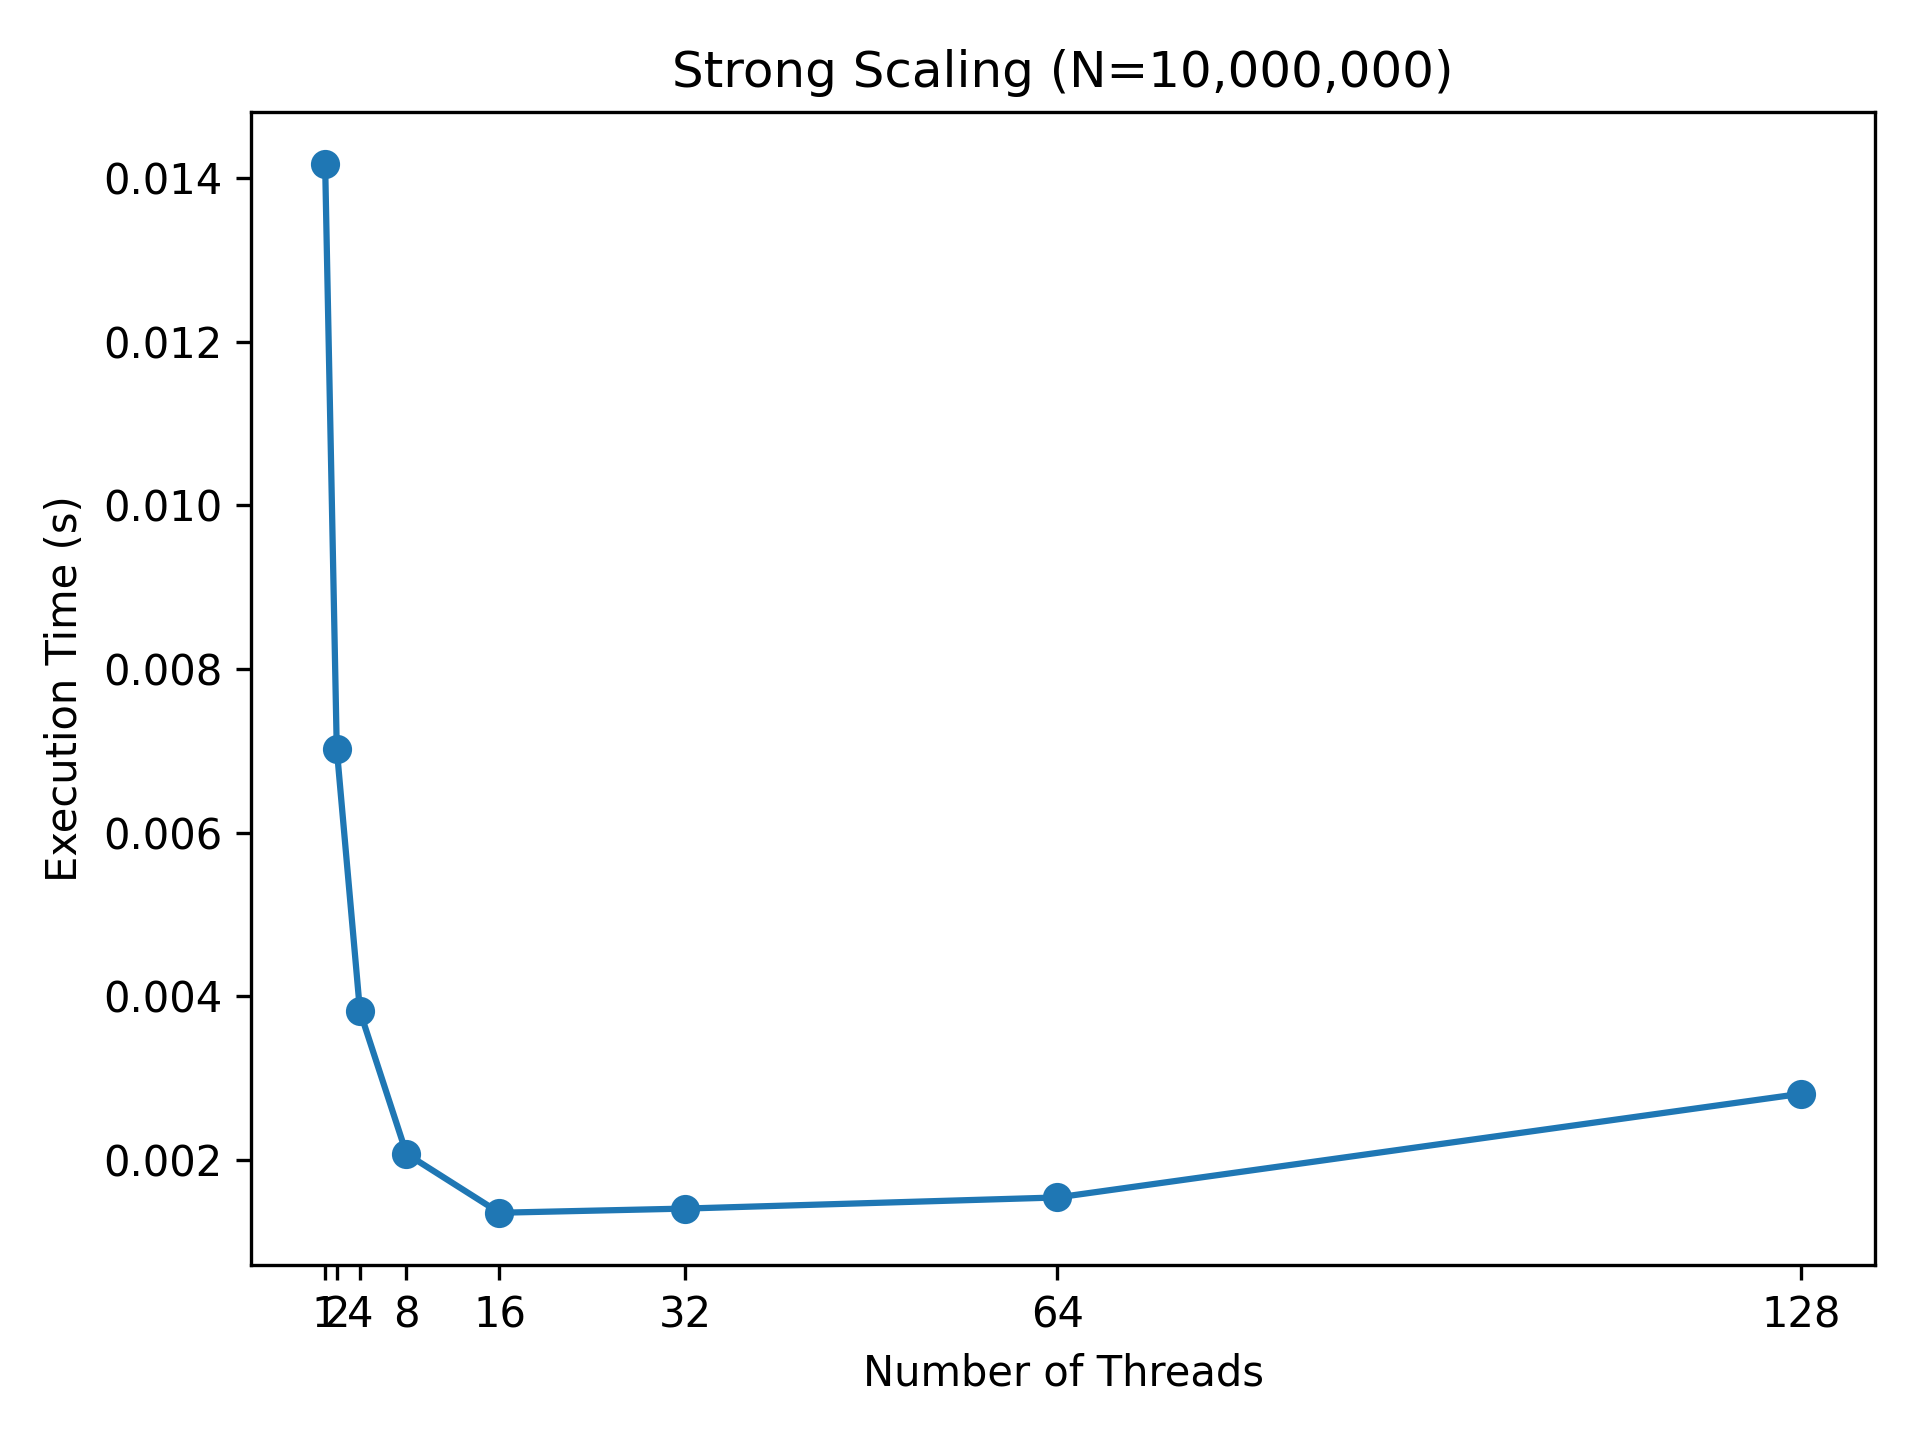
\includegraphics[width=0.45\textwidth]{plot_scaling.png}
\caption{Execution time vs number of threads.}
\end{figure}

Execution time decreases significantly as the number of threads increases up to around 16–32 threads. 
Beyond this point, performance improvements diminish due to increased synchronization overhead and memory contention.

\subsection{Scheduling Policies}

The final experiment compared static and dynamic scheduling with chunk sizes of 10, 100, and 1000.

\begin{figure}[h]
\centering
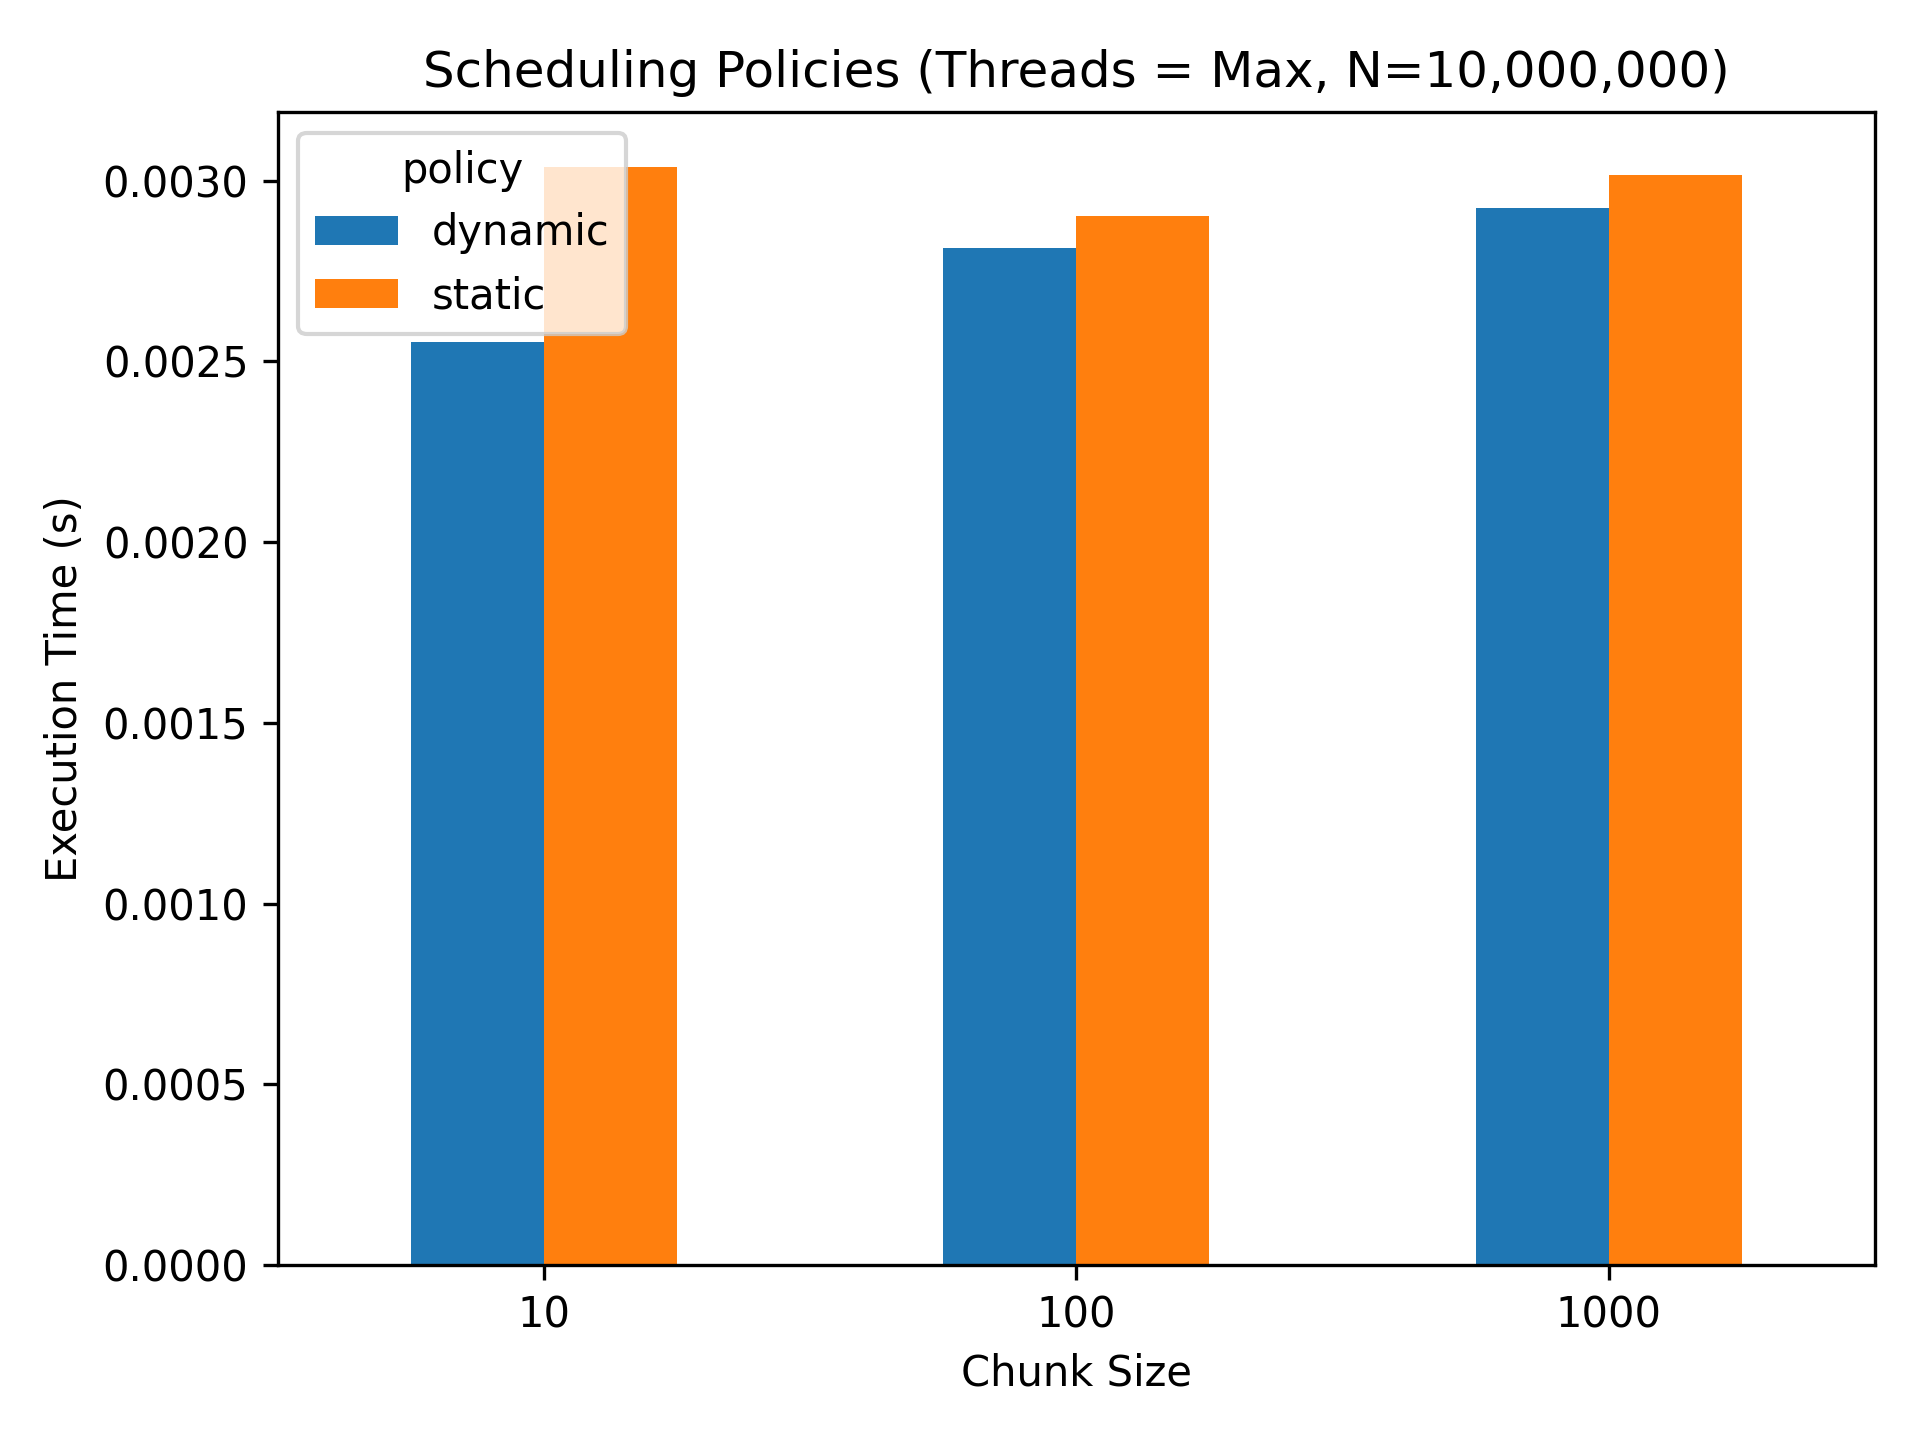
\includegraphics[width=0.45\textwidth]{plot_schedule.png}
\caption{Performance comparison of static and dynamic scheduling.}
\end{figure}

Dynamic scheduling produced slightly better performance because it allows threads to dynamically acquire new work, improving load balancing.

\section{Conclusion}

This assignment demonstrated how OpenMP can be used to parallelize a numerical computation and how runtime parameters influence performance.

The results show that:

\begin{itemize}
\item Thread placement significantly impacts performance on NUMA architectures.
\item Core-spread placement provided the best performance.
\item The application scales effectively up to moderate thread counts.
\item Dynamic scheduling slightly improves load balancing compared to static scheduling.
\end{itemize}

These findings highlight the importance of tuning OpenMP runtime parameters for achieving optimal performance in parallel applications.

\end{document}
